%%%%%%%%%%%%%%%%%%%%%%%%%%%%%%%%%%%%%%%%%%%%%%%%%%%%%%%%%%%% 
% This is the official template for theses and seminar papers from the Chair for Information Systems for Sustainable Society (IS3) at the University of Cologne

%
%PREAMBLE
%%%%%%%%%%%%%%%%%%%%%%%%%%%%%%%%%%%%%%%%%%%%%%%%%%%%%%%%%%%%%

\documentclass[a4paper, 12pt]{article}
\usepackage[utf8]{inputenc}

\usepackage{ragged2e}

% Font
\usepackage[T1]{fontenc}
\usepackage{tgtermes}
\usepackage{relsize}

\usepackage{color}
\usepackage{fifo-stack}
\FSCreate{colors}{black}
\makeatletter
\let\old@color\color
\renewcommand\color[1]{\FSPush{colors}{#1}\old@color{#1}}
\newcommand\colorend{\FSPop{colors}\old@color{\FSTop{colors}}}
\makeatother

\usepackage{graphicx}
\usepackage{longtable}
\usepackage{hyperref}
\usepackage{caption}

% Define blank page
% Use: \afterpage{\blankpage}
\usepackage{afterpage}
\newcommand\blankpage{%
    \null
    \thispagestyle{empty}%
    \addtocounter{page}{-1}%
    \newpage}


% set margins for double-sided printing
\usepackage[left=2.5cm, right=2.5cm, top=2.5cm, bottom=2.5cm, bindingoffset=1.5cm, head=15pt]{geometry} 
\usepackage{setspace}
\onehalfspacing

% set headers
\usepackage{fancyhdr}
\pagestyle{fancy}
\fancyhead{}
\fancyfoot{}

% \fancyhead[LO]{\textsl{\leftmark}} for two sided
\fancyhead[LO]{\rightmark \vspace{0.1cm}}
% \fancyhead[RO]{\leftmark \vspace{0.1cm}}
\fancyfoot[C]{\thepage}
\renewcommand{\headrulewidth}{0.6pt}
\renewcommand{\footrulewidth}{0pt}

% set APA citation style
% \usepackage{apacite}
\usepackage[numbib,notlof,nottoc, notlot]{tocbibind}
\pagenumbering{gobble}

% Reference management
\usepackage[
    backend=biber,
    style=numeric,
    sorting=ynt
]{biblatex}
\addbibresource{Bibliography.bib}

\usepackage{svg}

\hypersetup{pdfborder = {0 0 0}}

%%%%%%%%%%%%%%%%%%%%%%%%%%%%%%%%%%%%%%%%%%%%%%%%%%%%%%%%%%%%%
%THESIS Parameters 
%%%%%%%%%%%%%%%%%%%%%%%%%%%%%%%%%%%%%%%%%%%%%%%%%%%%%%%%%%%%%

\newcommand{\thesisdate}{September, 2020}
\newcommand{\thesisauthor}{Tojagi\'c Rastko} %input name
\newcommand{\studentID}{999999999} %input student ID
\newcommand{\thesistype}{

Informati\v{c}ki Projekat

} % Set either to Bachelor or Master
% \newcommand{\supervisor}{Univ.-Prof. Dr. Wolfgang Ketter}
% \newcommand{\cosupervisor}{Max Mustermann}



%%%%%%%%%%%%%%%%%%%%%%%%%%%%%%%%%%%%%%%%%%%%%%%%%%%%%%%%%%%%%
%DOCUMENT
%%%%%%%%%%%%%%%%%%%%%%%%%%%%%%%%%%%%%%%%%%%%%%%%%%%%%%%%%%%%%
\begin{document}

%%%%%%%%%%%%%%%%%%%%%%%%%%%%%%%%%%%%%%%%%%%%%%%%%%%%%%%%%%%%%
%TITLE PAGE (Pre-defined, just change parameters above)
%%%%%%%%%%%%%%%%%%%%%%%%%%%%%%%%%%%%%%%%%%%%%%%%%%%%%%%%%%%%%
%%%%%%%%%%%%%%%%%%%%%%%%%%%%%%%%%%%%%%%%%%%%%%%%%%%%%%%%%%%%%
%TITLE PAGE
%%%%%%%%%%%%%%%%%%%%%%%%%%%%%%%%%%%%%%%%%%%%%%%%%%%%%%%%%%%%%

\newgeometry{
 a4paper,
 total={170mm,257mm},
 left=20mm,
 top=26mm,
}

\begin{titlepage}
    \noindent% just to prevent indentation narrowing the line width for this line
    
\includegraphics[width=0.18\textwidth]{Figures/pmf_logo.png}%
    \begin{minipage}{0.6\textwidth}
        \Large
        \centering
        \vspace{-2.8cm}
        \textsc{
            \vspace{-0.4cm}
            univerzitet u novom sadu
            \vspace{-0.3cm}
            prirodno-matemati\v{c}ki fakultet
            \vspace{-0.4cm}
            departman za matematiku i informatiku
        }
    \end{minipage}%
    
\includegraphics[width=0.18\textwidth]{Figures/uni_logo.png}
    \begin{center}
        \vspace*{5cm}

        \LARGE
        \textbf{\@
            \begin{minipage}{0.86\textwidth}
                \centering
                Svemirska puca\v{c}ina "Andromeda" \\ 
                u Unity platformi
            \end{minipage}%
        }

        \vspace{1.6cm}
        
        \Large
        \thesistype{}
        
        \vspace{0.2cm}

        \large
        %\textbf{Author}: \thesisauthor{} (Student ID: \studentID{})\\
        Tojagi\'c Rastko
        \large
        %\textbf{Supervisor}: \supervisor{}\\
        \large
        %\textbf{Co-Supervisor}: \cosupervisor{}

        % \large
        % Department of Information Systems for Sustainable Society\\
        % Faculty of Management, Economics and Social Sciences\\
        % University of Cologne\\

        % \vspace{1cm}
        % \@date
        
        \vspace{9cm}
        \textbf{Novi Sad, 2020.}

    \end{center}
\end{titlepage}

\makeatother

\afterpage{\blankpage}

\clearpage

\restoregeometry

\relscale{1.1}

%%%%%%%%%%%%%%%%%%%%%%%%%%%%%%%%%%%%%%%%%%%%%%%%%%%%%%%%%%%%%
%SOOA
%%%%%%%%%%%%%%%%%%%%%%%%%%%%%%%%%%%%%%%%%%%%%%%%%%%%%%%%%%%%%
% \clearpage
\thispagestyle{empty}
\section*{Eidesstattliche Versicherung}
\label{sec:SOOA}

\vspace{2.5cm}

% Statement of original authorship - Needs to be in German
% see also here: https://www.wiso.uni-koeln.de/sites/fakultaet/dokumente/PA/formulare/eidesstattliche_erklaerung.pdf

Hiermit versichere ich an Eides statt, dass ich die vorliegende Arbeit selbstständig und ohne die Benutzung anderer als der angegebenen Hilfsmittel angefertigt habe. Alle Stellen, die wörtlich oder sinngemäß aus veröffentlichten und nicht veröffentlichten Schriften entnommen wurden, sind als solche kenntlich gemacht. Die Arbeit ist in gleicher oder ähnlicher Form oder auszugsweise im Rahmen einer anderen Prüfung noch nicht vorgelegt worden. Ich versichere, dass die eingereichte elektronische Fassung der eingereichten Druckfassung vollständig entspricht.

\vspace{1cm}

\noindent
Die Strafbarkeit einer falschen eidesstattlichen Versicherung ist mir bekannt, namentlich die Strafandrohung gemäß § 156 StGB bis zu drei Jahren Freiheitsstrafe oder Geldstrafe bei vorsätzlicher Begehung der Tat bzw. gemäß § 161 Abs. 1 StGB bis zu einem Jahr Freiheitsstrafe oder Geldstrafe bei fahrlässiger Begehung.

\vspace{3cm}
\noindent
\textbf{\thesisauthor{}} 

\vspace{0.5cm}
\noindent
Köln, den xx.xx.20xx


%%%%%%%%%%%%%%%%%%%%%%%%%%%%%%%%%%%%%%%%%%%%%%%%%%%%%%%%%%%%%
%ABSTRACT
%%%%%%%%%%%%%%%%%%%%%%%%%%%%%%%%%%%%%%%%%%%%%%%%%%%%%%%%%%%%%
\clearpage
\justify
\thispagestyle{empty}
\section*{Predgovor}

Razvoj ra\v{c}unarskih igara je tokom protekle decenije veoma uznapredovao zahvaljuju\'ci pojavi
platformi koje taj razvoj znatno olak\v{s}avaju i ubrzavaju. Jedna od takvih platformi jeste Unity koji
podr\v{z}ava razvoj kako jednostavnijih 2d tako i zahtevnijih 3d igara. U ovom informati\v{c}kom projektu
pokaza\'cemo upravo koliko je jednostavno napraviti 2d svemirsku puca\v{c}inu u svega nekoliko stotina
linija koda, kao i neke \v{c}esto kori\v{s}\'cene obrasce (eng. design patterns) u razvoju igara.

\vspace{3cm}
\noindent
\textbf{\thesisauthor{}} 

\vspace{0.2cm}
\noindent
Novi Sad, Septembar 2020.


%%%%%%%%%%%%%%%%%%%%%%%%%%%%%%%%%%%%%%%%%%%%%%%%%%%%%%%%%%%%%
%TOC,TOF,TOT
%%%%%%%%%%%%%%%%%%%%%%%%%%%%%%%%%%%%%%%%%%%%%%%%%%%%%%%%%%%%%
\clearpage
\renewcommand{\contentsname}{Sadr\v{z}aj}
\pagenumbering{Roman}
\tableofcontents
\clearpage
% \listoffigures
% \clearpage
% \listoftables
% \clearpage

\pagenumbering{arabic}


%%%%%%%%%%%%%%%%%%%%%%%%%%%%%%%%%%%%%%%%%%%%%%%%%%%%%%%%%%%%%
%MAIN PART
%%%%%%%%%%%%%%%%%%%%%%%%%%%%%%%%%%%%%%%%%%%%%%%%%%%%%%%%%%%%%

% SEC1
\clearpage
\section{Platforma za razvoj igara Unity}

\subsection{MonoBehaviour i pisanje skripti u jeziku C\#}

\emph{MonoBehaviour} je osnovna klasa koju svaka Unity skripta nasle\v{dj}uje. Kada
koristimo C\# za skriptni jezik ovu klasu moramo eksplicitno da nasledimo \cite{unitydocs}. U svakom trenutku
mogu\'ce je isklju\v{c}iti ili ponovo uklju\v{c}iti skriptu. Isklju\v{c}ivanje
izuzima skriptu iz aktivnih skripti. Ukoliko je skripta uklju\v{c}ena i ima definisane
neke od specifi\v{c}nih funkcija koje se pozivaju u odre\dj enom trenutku tokom
\v{z}ivotnog ciklusa objekta smatra se aktivnom i reaguje na pozive tih funkcija
onako kako je korisnik to definisao. Neke od klju\v{c}nih funkcija su: \emph{Start()}, \emph{Update()},
\emph{FixedUpdate()}, \emph{OnEnable()}, \emph{OnDisable()}. \v{Z}ivotni ciklus skripte prikazan
je grafikonom ~\ref{fig:monoflowchart}. Kasnije u tekstu bi\'ce data preciznija obja\v{s}njenja
za najbitnije funkcije.

Drugim re\v{c}ima MonoBehaviour predstavlja definisano pona\v{s}anje nekog \v{z}ivog objekta
u svetu igre. Svaki objekat u svetu igre naziva se \emph{GameObject} i tipa je istoimene klase. Svaki
MonoBehaviour jeste \emph{GameObject}. Na GameObject je mogu\'ce dodati komponente. Treba imati 
na umu da ovakav sistem koji Unity pru\v{z}a nije pravi ECS (Entity Component System) te da zbog ovakvog
dizajna cela platforma radi sporije. Unity od skoro uvodi pravi ECS uz \emph{Burst Compiler}, ali ovo jo\v{s} uvek 
nije deo standardne platforme \cite{unitydocs}.

\begin{center}
    \begin{figure}
        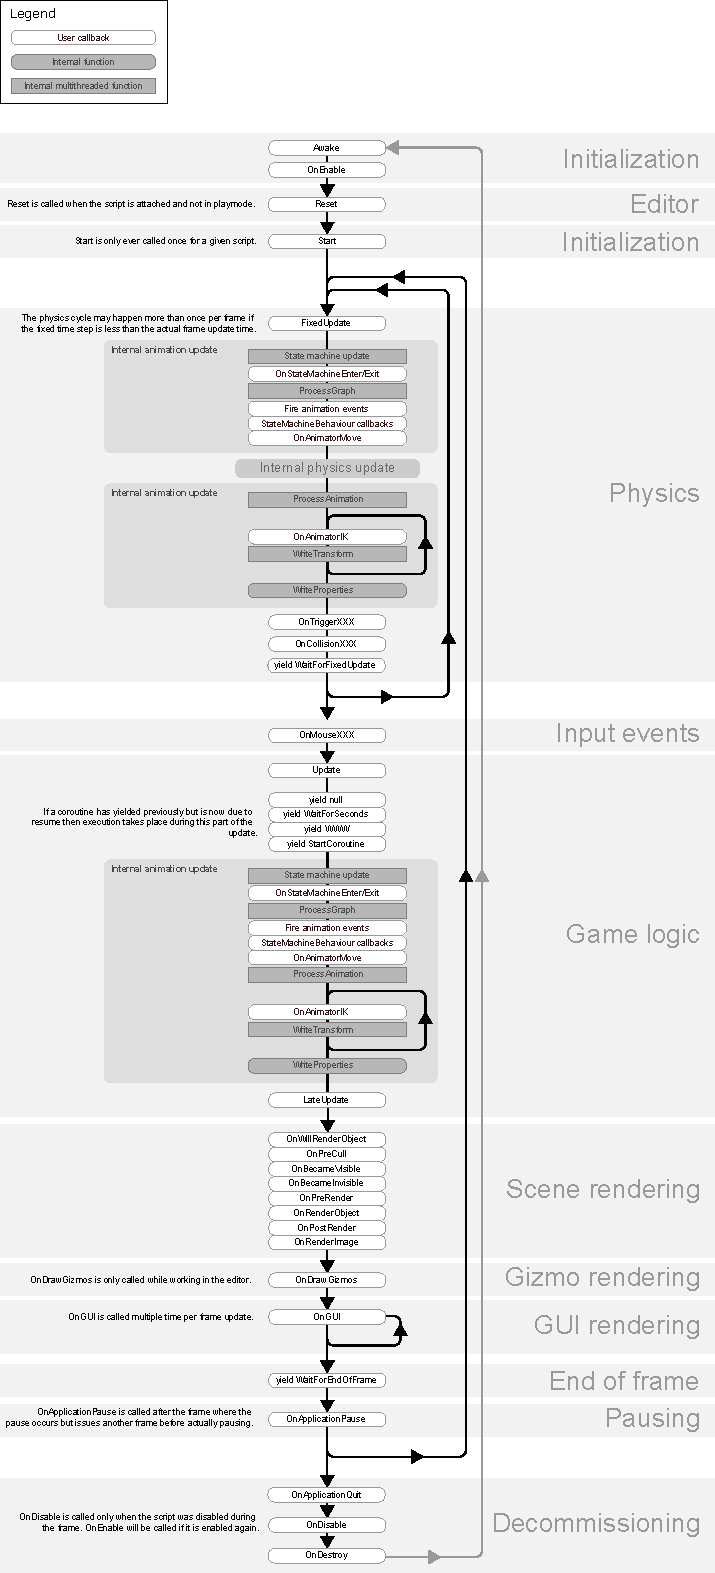
\includegraphics[width=0.7\textwidth]{Figures/mono_flowchart.pdf}
        \caption{MonoBehaviour lifecycle}
        \label{fig:monoflowchart}
    \end{figure}
\end{center}

\subsection{Unity Editor}

Editor ~\ref{fig:unityeditor} je grafi\v{c}ko okru\v{z}enje namenjeno za postavljanje sveta igre. Editor
pru\v{z}a vizuelni pregled svih objekata na sceni, kamere i efekata. Prozor je podeljen
na nekoliko potprozora \v{c}ije uloge su da olak\v{s}aju pode\v{s}avnja i pregled igre.

\emph{SceneView} predstavlja pregled trenutne, aktivne scene. Scena predstavlja skup
objekata i kameru koji su u datom trenutku prikazani korisniku. Po\v{z}eljno je zasebne
logi\v{c}ke celine igre odvajati u zasebne scene, tako na primer, mo\v{z}emo imati scenu
za \emph{glavni meni} i \emph{scenu igre}, gde bi kroz u meniju bila omogu\'cena neka pode\v{s}avanja,
pregled najboljih rezultata i sli\v{c}no, dok je scena igre sama igra.

\emph{Hierarchy View} omogu\'cava pregled svih objekata na trenutnoj sceni. Objekti mogu
biti u roditelj-dete odnosu, te stoga i ime, jer tako \v{c}ine hijerarhiju.

\emph{Project View} daje pregled svih fajlova trenutno otvorenog projekta na disku.

\emph{Game View} obi\v{c}no slo\v{z}en pored pregleda scene prikazuje svet igre
onakav kakav \'ce biti prikazan igra\v{c}u, dakle bez pomo\'cnih elemenata poput 
kvadratne mre\v{z}e ili mogu\'cnosti pomeranja objekata. 

\begin{center}
    \begin{figure}
        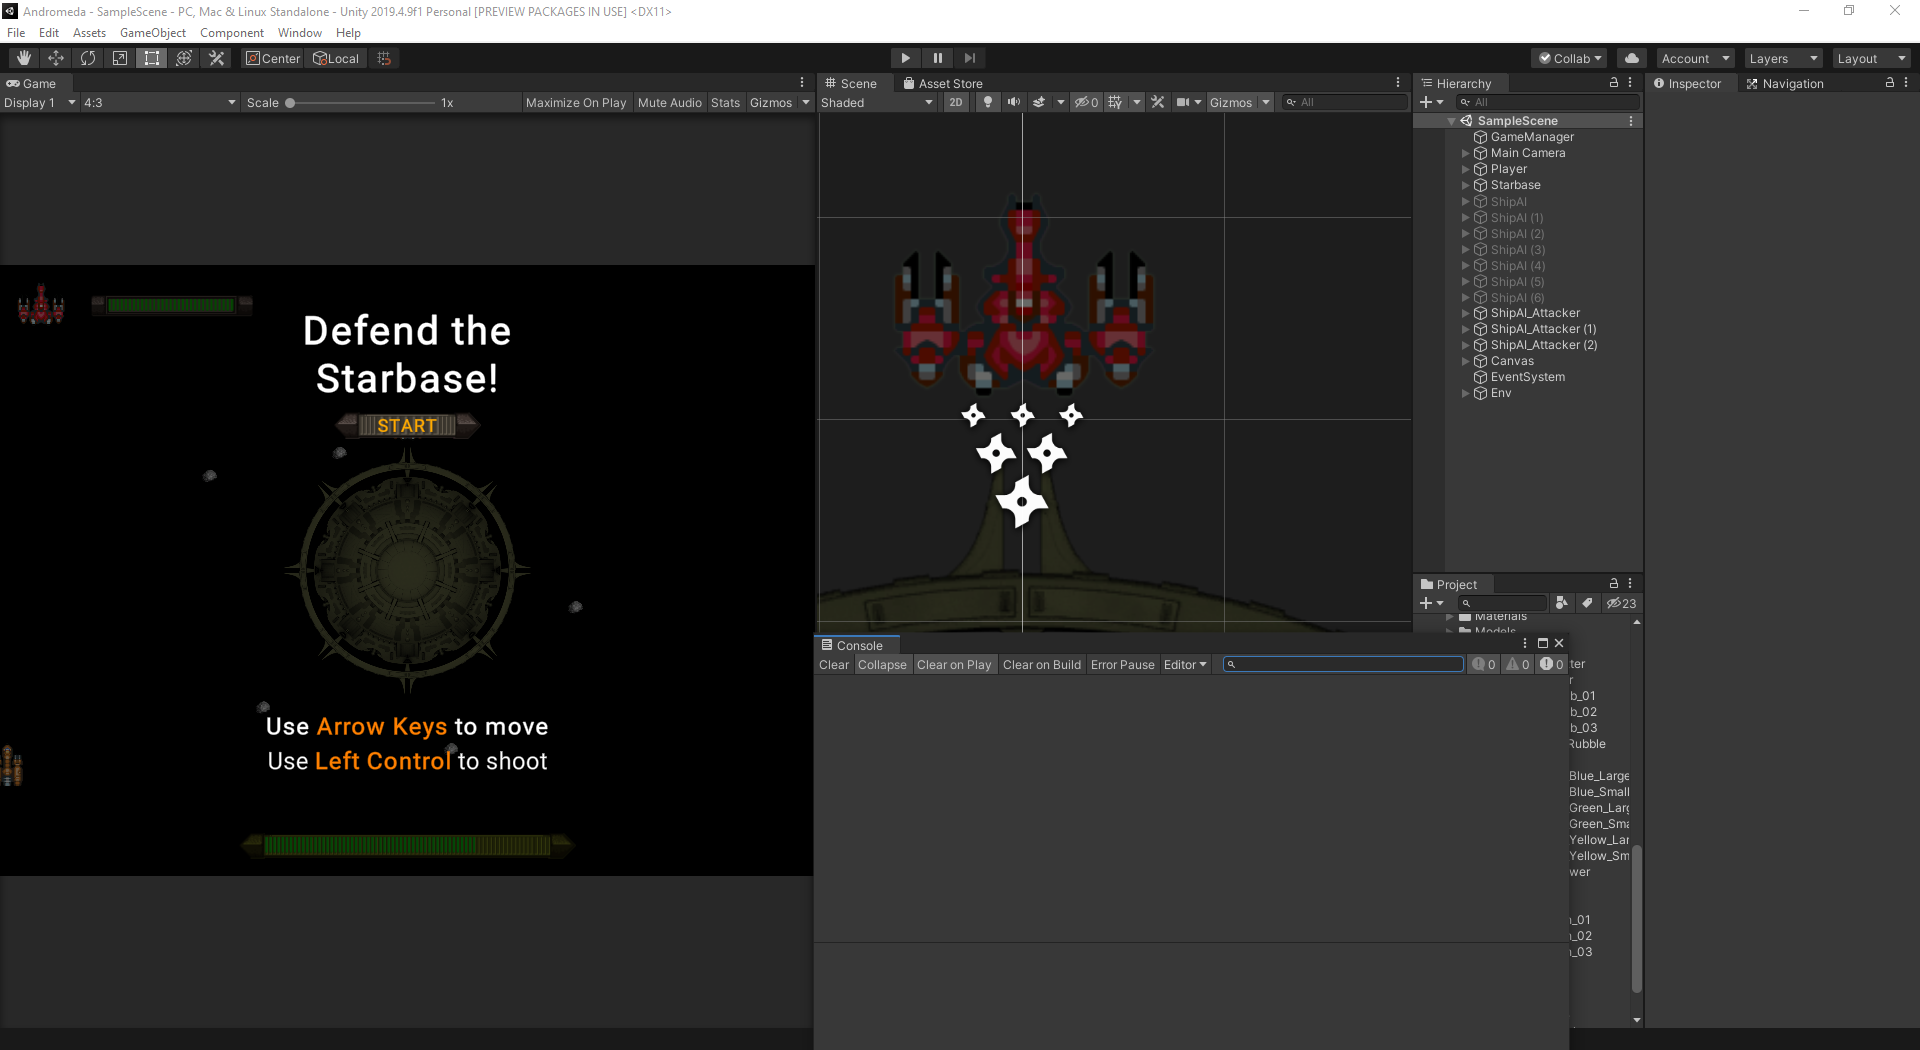
\includegraphics[width=1\textwidth]{Figures/Editor.png}
        \caption{Unity Editor}
        \label{fig:unityeditor}
    \end{figure}
\end{center}

% \label{sec:Intro}
% ...

% \subsection{Exemplary Table}
% \label{subsec:Intro/table}
% ...

% \begin{longtable}{l|ccccc}
%   \caption{Exemplary Table}
%   \label{table:table-1}
%   \\
%   \textbf{Id} & \textbf{Col 1} & \textbf{Col 2}& \textbf{Col 3} & \textbf{Col 4} & \textbf{Col 5}\\
%   \hline
%   1 & Col 1 & Col 2 & Col 3 & Col 4 & Col 5\\
%   2 & Col 1 & Col 2 & Col 3 & Col 4 & Col 5\\
%   3 & Col 1 & Col 2 & Col 3 & Col 4 & Col 5\\
%   4 & Col 1 & Col 2 & Col 3 & Col 4 & Col 5\\
%   5 & Col 1 & Col 2 & Col 3 & Col 4 & Col 5\\
% \end{longtable}

% \subsection{Exemplary Section and Table Referencing}
% \label{subsec:Intro/rfs}

% See Table \ref{table:table-1} in Section \ref{subsec:Intro/table}  for details.

% SEC2
\clearpage
\section{Osnovni pojmovi i sistemi u igrama}
\label{sec:Section_Name}

\subsection{Game Loop}
Klju\v{c}na ta\v{c}ka izvr\v{s}avanja igre jeste glavna petlja igre (eng. game loop).
Jednom kada je igra pokrenuta sve ono \v{s}to je vidljivo korisniku, grafika, 
zvuk, interakcija procesira se kroz glavnu petlju. U tom jednom prolazu petlje koji
nazivamo \emph{tick} ili \emph{frame} de\v{s}ava se iscrtavanje grafike, reagovanje na 
korisni\v{c}ki unos (unos sa tastature ili putem mi\v{s}a ili nekih drugih perifernih ure\dj aja) 
te reakcija sveta na zadate promene... odnosno, ovde se de\v{s}ava sve, zato je glavna 
petlja srce same igre. Modernije arhitekture dozvoljavaju odre\dj eni stepen paralelizacije
nekih procesa, pa bi na primer iscrtavanje grafike moglo da se izdvoji u paralelan proces i sli\v{c}no.

\subsubsection{FPS}
FPS skra\'ceno od \emph{frames per second} je osnovna mera performansi igre. Ova mera kazuje nam
koliko je puta po sekundi mogu\'ce izvr\v{s}iti glavnu petlju. Ve\'ci broj je i bolji, pa tako igra
koja se izvr\v{s}ava na manje od 30 frejmova po sekundi nije prijatna za igranje
i doga\dj a se takozvano \emph{seckanje}, odnosno objekti se ne pomeraju glatko kako bi trebalo
ve\'c iscepkano \v{s}to naru\v{s}ava celokupan do\v{z}ivljaj igranja. Nizak FPS mo\v{z}e
da bude rezultat lo\v{s}e napisanog koda ili prosto zastarelog hardvera. Moderne igre se trude da 
se odr\v{z}e na 60 FPS.

\subsubsection{Update}
Update je funkcija koja se poziva upravo iz glavne petlje igre. To je funkcija koja je mo\v{z}e biti
definsana u MonoBehavior klasi. Update funkcija se poziva nad svakim objektom tipa MonoBehavior (ukoliko
je defini\v{s}e) ta\v{c}no jednom svakog frejma \cite{unitydocs}. Sva promenljiva pona\v{s}anja objekta
mogu se definisati ovde.

\subsubsection{FixedUpdate}
Sli\v{c}no funkciji Update, i ova funkcija se poziva periodi\v{c}no ali ne svakog frejma, ve\'c 
na fiksno vreme svake 0.02 sekunde \cite{unitydocs}. Prema uputstvima iz dokumentaicje,
u ovoj funkciji se mora raditi sve \v{s}to ima veze sa bilo kakvim izra\v{c}unavanjem fizike. U igri
se oslanjamo na Unity-jev sistem za fiziku za kretanje, pa \'cemo se dalje u tekstu detaljnije
baviti time.

\subsubsection{Vremena, klasa Time}
Jedna od bitnijih stavki u igrama jeste vreme. Merimo dve vrste vremena, koja o\v{c}itavamo iz klase \emph{Time}.

\emph{Time.time} je vreme koje je proteklo od pokretanja igre i ono je korisno
obi\v{c}no kada \v{z}elimo da ograni\v{c}imo izvr\v{s}avanje nekog dela koda vremenski.
Na primer, ne \v{z}elimo da neprijatelji prebrzo ispaljuju metke na igra\v{c}a, te mo\v{z}emo meriti
vreme proteklo od prethodnog pucanja i proveriti da li je to vreme ve\'ce od neke konstante
koja nam predstavlja minimalan vremenski interval izme\dj u dva pucnja.

\emph{Time.deltaTime} je vreme za koje se izvr\v{s}io prethodni frejm. Ovo je jako bitna stavka,
i potrebno nam je kada imamo bilo kakvo kretanje u igri. \color{red} ** TODO: Ubaciti grafik koji objasnjava vaznost mnozenja vrednosti kretanja sa deltatime **

\colorend


\subsection{Obrasci (eng. design patterns)}
\subsubsection{"Singleton" obrazac}
\subsubsection{"Command" obrazac}


% SEC X
\clearpage
\section{Andromeda - Svemirska puca\v{c}ina}
\label{sec:Section_Name_X}

\subsection{Pregled i ideja igre}

\subsection{GameManager klasa}

\subsection{Kontrole}

\subsection{Pona\v{s}anje svemirskog broda i ShipController klasa}

\subsection{Neprijatelji i osnovno pona\v{s}anje}

\subsection{Pobolj\v{s}anja i optimizacije}

%%%%%%%%%%%%%%%%%%%%%%%%%%%%%%%%%%%%%%%%%%%%%%%%%%%%%%%%%%%%%
%APPENDICES
%%%%%%%%%%%%%%%%%%%%%%%%%%%%%%%%%%%%%%%%%%%%%%%%%%%%%%%%%%%%%


% \appendix
% \renewcommand*{\thesection}{\Alph{section}}\textbf{}

% APPENDIX A
% \clearpage
\section{Appendix}
\label{app:A}
...

%%%%%%%%%%%%%%%%%%%%%%%%%%%%%%%%%%%%%%%%%%%%%%%%%%%%%%%%%%%%%
%BIBLIOGRAPHY
%%%%%%%%%%%%%%%%%%%%%%%%%%%%%%%%%%%%%%%%%%%%%%%%%%%%%%%%%%%%%
\printbibliography

\end{document}